\section{集合与集合运算}
\label{sec:01-Mathematical-Language/02-Sets-Relations-Functions/01}

两个人各交了一份``本月活跃用户 ID''的去重清单。一份写着 \(\{1,2,3\}\)，另一份写着 \(\{3,2,1,2\}\)。核对的时候，这两份算不算一致？

按文本比，第二份显然不一样：多了一个 2，顺序也乱了。但换个问法——``哪些 ID 出现在清单里''——两份的答案逐字相同：1 在、2 在、3 在，别的都不在。2 被写了两遍，不会因此多出一个用户。

集合采用后一种比法。这条约定叫外延性：两个集合相等，当且仅当它们的元素完全一样。

\[
\{1,2,2,3\}=\{3,2,1\}.
\]

接受外延性，就得同时接受它的代价：集合不记顺序，也不记重复次数。这不是缺陷，是选型。要问``用户按什么顺序访问了这些页面''，集合是错的容器，该用序列 \((a_1,a_2,\ldots)\)；要问``每个页面被访问了多少次''，该用多重集（multiset）——允许元素重复并记录次数的结构。把访问日志直接塞进一个集合，第一步就把频次扔了，后面再精巧的推导也捞不回来。选容器就是在选你打算保留哪些信息。

\subsection{元素与子集是两种不同的关系}

\(x\in A\) 说的是 \(x\) 是 \(A\) 的一个成员，一头是对象一头是容器；\(A\subseteq B\) 说的是 \(A\) 的每个成员也都是 \(B\) 的成员，两头都是容器。写成逻辑就一目了然：

\[
A\subseteq B
\quad\Longleftrightarrow\quad
\forall x,(x\in A\to x\in B).
\]

麻烦出在元素本身也可以是集合的时候。设 \(A=\{1,\{2\}\}\)，它有两个成员：数字 1，以及集合 \(\{2\}\)。

\begin{center}
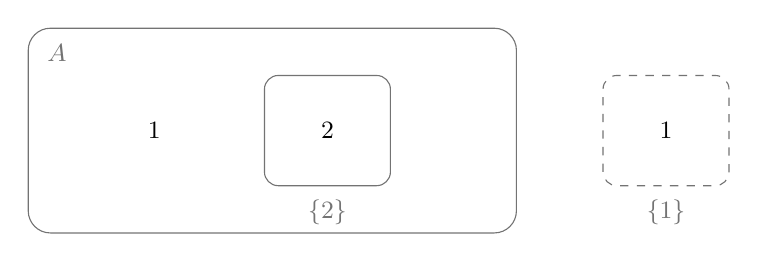
\begin{tikzpicture}[font=\small]
  \draw[rounded corners=8pt,black!55] (0,0) rectangle (6.2,2.6);
  \node[anchor=north west,black!55] at (0.12,2.52) {\(A\)};
  \node at (1.6,1.3) {\(1\)};
  \draw[rounded corners=5pt,black!55] (3.0,0.6) rectangle (4.6,2.0);
  \node at (3.8,1.3) {\(2\)};
  \node[anchor=north,black!55] at (3.8,0.55) {\(\{2\}\)};
  \draw[dashed,rounded corners=5pt,black!55] (7.3,0.6) rectangle (8.9,2.0);
  \node at (8.1,1.3) {\(1\)};
  \node[anchor=north,black!55] at (8.1,0.55) {\(\{1\}\)};
\end{tikzpicture}

\emph{\(A\) 里装着两样东西：一个裸的数字 1，和一个装着 2 的盒子。数字 2 躲在内层盒子里，不是 \(A\) 的成员；右边那个``装着 1 的盒子''压根不在 \(A\) 里，所以 \(\{1\}\notin A\)，但 \(\{1\}\subseteq A\)。}
\end{center}

于是 \(1\in A\) 和 \(\{2\}\in A\) 都成立，\(2\in A\) 却不成立——\(A\) 里没有裸的数字 2。同理，\(\{1\}\subseteq A\) 成立（它唯一的元素 1 确实在 \(A\) 里），\(\{1\}\in A\) 不成立。花括号是一层包装纸，拆一层和不拆是两码事。

空集 \(\varnothing\) 一个元素都没有，却是任何集合的子集：\(\varnothing\subseteq B\) 要求 \(\forall x(x\in\varnothing\to x\in B)\)，而前件 \(x\in\varnothing\) 永远为假，蕴含自动成立。这正是上一章那条``前提未触发就不构成反例''的规则在集合里的第一次应用。顺带一提，\(\varnothing\) 与 \(\{\varnothing\}\) 不是一回事：后者是装了一个空盒子的盒子，有一个元素。

证明两个集合相等的标准路线也由此确定：先证 \(A\subseteq B\)，再证 \(B\subseteq A\)。比的是元素的归属，不是两段描述文字读起来像不像。

\subsection{集合运算是逻辑的改写}

三个基本运算的定义摆在一起，对应关系就藏不住了：

\[
\begin{aligned}
A\cup B&=\{x:x\in A\lor x\in B\},\\
A\cap B&=\{x:x\in A\land x\in B\},\\
A\setminus B&=\{x:x\in A\land x\notin B\}.
\end{aligned}
\]

并用``或''，交用``且''，差用``且不''。认出这层对应，所谓的集合恒等式就不必单独去记——它们都是上一章的逻辑等价式换了一套符号。

补集 \(A^{c}=U\setminus A\) 要先固定全集 \(U\)，否则无从谈起。同一个 \(A=\{1,2\}\)，在 \(U=\{1,2,3,4\}\) 里补集是 \(\{3,4\}\)，在 \(U=\Z\) 里补集是除 1 和 2 之外的全体整数。每次写补集，先确认全集是谁。

De Morgan 律照搬过来：

\[
(A\cup B)^{c}=A^{c}\cap B^{c},
\qquad
(A\cap B)^{c}=A^{c}\cup B^{c}.
\]

验证第一式，任取 \(x\)：

\[
\begin{aligned}
x\in(A\cup B)^{c}
&\Longleftrightarrow \neg(x\in A\lor x\in B)\\
&\Longleftrightarrow x\notin A\land x\notin B\\
&\Longleftrightarrow x\in A^{c}\cap B^{c}.
\end{aligned}
\]

第一步和第三步是补集的定义，中间那步是逻辑的 De Morgan 律。全程只是在成员资格的是与否之间来回翻译。

现实中的筛选规则就是这种翻译的直接用途。以一项临床研究的入组为例：全集 \(U\) 是所有到诊患者，\(A\) 是年龄符合的，\(C\) 是已签知情同意的，\(B\) 是有禁忌症的，可纳入人群写作

\[
(A\cap C)\setminus B.
\]

这行式子的价值不在于短——换成三句自然语言同样短——而在于它逼你把每项标准的边界先定死。``年龄符合''是 \(\ge 18\) 还是 \(\ge 21\)？``有禁忌症''以病历记录为准还是以患者自述为准？成员资格的检验规则不先定下来，交并补算得再漂亮也不作数。

这里还埋着一个符号运算永远查不出来的错误。如果数据库里``禁忌症字段为空''被当成了``确认没有禁忌症''，那么 \(B\) 从一开始就装错了人，而 \((A\cap C)\setminus B\) 会照算不误。集合代数保证的是运算正确，不保证成员资格的定义正确。

同一条警戒线也划在描述法上。\(\{x\in U:\varphi(x)\}\) 只有当 \(\varphi\) 对每个 \(x\) 都能判定真假时才定义了一个集合；把``美丽的''这种没有检验规则的谓词塞进去，得到的不是集合，只是一串带花括号的装饰。真正带渐进性的成员资格（一个人算不算高收入群体）需要模糊集合那套工具，它承认成员度是 \(0\) 到 \(1\) 之间的数，不在本章范围内。最后，也不是所有能用语言描述的聚合都能当集合——``所有不以自身为元素的集合''会直接引出罗素悖论。朴素集合论在绝大多数场合够用，但要知道边上有这么一条线。

\subsection{幂集：把子集本身当成元素}

既然元素可以是任何东西，那就把 \(A\) 的所有子集收集起来当成一个新集合：

\[
\mathcal P(A)=\{B:B\subseteq A\}.
\]

取 \(A=\{a,b\}\)，枚举得 \(\mathcal P(A)=\{\varnothing,\{a\},\{b\},\{a,b\}\}\)。这里 \(\varnothing\in\mathcal P(A)\) 和 \(\varnothing\subseteq\mathcal P(A)\) 同时成立，理由却不同：前者因为 \(\varnothing\subseteq A\)，后者因为空集是任何集合的子集。

幂集为什么恰有 \(2^{n}\) 个元素（\(n\) 是 \(A\) 的元素个数，记作 \(\abs{A}\)）？构造一个子集时，对每个元素独立地做一次二选一：要它，或者不要它。\(n\) 次独立的二选一给出 \(2^{n}\) 种结果，而不同的选法给出不同的子集。这个``对每个特征选或不选''的计数模式，后面在组合计数和特征子集搜索里还会一再出现。

Cantor 把它推到了无限：即便 \(A\) 是无限集，也不存在从 \(A\) 到 \(\mathcal P(A)\) 的满射，无论配对规则设计得多精巧，总有子集被漏掉。``满射''的定义见本章 \hyperref[sec:01-Mathematical-Language/02-Sets-Relations-Functions/04]{``函数与可逆性''}。它的推论是：无限不止一种大小。

\subsection{笛卡尔积：顺序合法入场}

集合一路拒绝记录顺序，笛卡尔积给顺序开了一扇门：

\[
A\times B=\{(a,b):a\in A,\; b\in B\}.
\]

有序对的相等标准是逐位相等，\((a,b)=(a',b')\) 当且仅当 \(a=a'\) 且 \(b=b'\)。所以一般 \(A\times B\ne B\times A\)，就像经纬度调换之后指向的是另一个地方。

学生集合 \(S=\{\text{张三},\text{李四}\}\) 与课程集合 \(C=\{\text{数学},\text{物理}\}\) 的笛卡尔积有四个元素，穷举了所有``学生—课程''配对。而真实的选课记录——张三只选数学，李四两门都选——只占其中三个。这个差额就是下一节的起点：从所有可能的配对里挑出确实成立的那些，挑出来的子集就叫关系。
